%% main.tex
%% Distributed with umalayathesis v1.5 (28 October 2018)
\documentclass[english,singlespacedlisttitles]{umalayathesis}
%% Document class options
%% -----------------------
%% english (default): English thesis
%%
%% bahasam : Malay thesis
%%
%% apacite (default): Loads the apacite package, which implements the APA
%%    citation and referencing styles strictly, including expansion of
%%    of 3–5 authors on first citation.
%%
%% newapa: Loads the natbib and apalike package for a APA-like reference list
%%    but *does not fully implement* all APA citation styles. In particular,
%%    this option will not expand references with 3–5 authors on first citation.
%%    NOT RECOMMENDED UNLESS EXPLICITLY REQUESTED BY EXAMINER.
%%
%% custombib: Does not pre-load any bibliography style; you will need to
%%    specify \bibliographystyle, \bibliographystyleown etc yourself.
%%
%% appendixhead: Add "APPENDICES" before the Appendix A title
%%
%% altcaption: Caption in smaller fonts; only Figure X, Table Y bold.
%%
%% singlespacedlisttitles: Long titles in the ToC, LoT, LoF, LoA are single-spaced.
%%
%% listpageheader: If your faculty requires a "header row" at the top of
%%    the List of Figures/Tables. You can re-define \lofpageheader and
%%    \lotpageheader if necessary, e.g.
%%           \renewcommand{\lofpageheader}{\hfill Page}
%%
%% boldfrontmattertoc: If your faculty wants front matter "chapters" to be
%%    bold in the ToC
%%
%% boldbackmattertoc: If the backmatter "chapters" are to be bolded as well
%%
%% uppercasetoc: If all "chapter" level headings must be upper-cased in the ToC

\usepackage{lipsum}
\usepackage[utf8]{inputenc}
\usepackage[T1]{fontenc}
\usepackage{microtype}
\usepackage{graphicx}
\usepackage{caption}
\usepackage[dvipsnames,x11names]{xcolor}
\usepackage{listings}
\usepackage{glossaries}

% For the process flow diagram in chapter 3
\usepackage{tikz}
\tikzstyle{block} = [rectangle, draw, fill=blue!20, text width=10em, text centered, rounded corners, minimum height=4em]
\tikzstyle{line} = [draw, -latex]

% Useful for including code listings
\usepackage{listings}
\lstset{language=[LaTeX]TeX,columns=fullflexible,
        basicstyle=\ttfamily\SingleSpacing,
        texcsstyle=*\bfseries\color{NavyBlue},
        commentstyle=\itshape\color{PaleVioletRed4},
        frame=single,framesep=6pt,
        framexleftmargin=6pt,framexrightmargin=6pt,
        xleftmargin=12pt,xrightmargin=12pt,
        breaklines=true,breakatwhitespace=true,
        aboveskip=-1.5\onelineskip
}

% Useful for multi-page pages. Either longtable or supertabular is fine; choose any one that you're comfortable with
\usepackage{longtable}
% \usepackage{supertabular}


\author{Ng Kang Wei}
\title{Text Classification with Dimension Reduction on News Articles}

%% If \othertitle is given, then the second abstract will display it
%% (i.e. if your thesis is "english" then this is printed on top of the Malay abstract
%% and if your thesis is "bahasam" then this is printed on top of the English abstract)
%% If no \othertitle is given then the second abstract will not have any translated thesis title
%\othertitle{Tajuk dalam Bahasa Lain untuk Abstrak Kedua}

\faculty{Department of Computer Science and Information Technology}
\submissionyear{2019}
\degree{Master of Data Science}

% load acronym definitions from separate file
\makeglossaries
\loadglsentries[acronym]{myacronyms}


\begin{document}
\frontmatter

%% Choose only ONE from the following to get the
%% correct statement on the title page
\makecoverandtitlepage{\mastercoursework}
% \makecoverandtitlepage{\mastermixedmode}
% \makecoverandtitlepage{\masterresearch}
% \makecoverandtitlepage{\doctoralcoursework}
% \makecoverandtitlepage{\doctoralresearch}
% \makecoverandtitlepage{\doctoralmixedmode}

\declarationpage
\abstractfromfile{abstract}
\msabstractfromfile{abstractms}
\acknowledgements{
	I would like to take this opportunity to appreciate the helps and guidance given freely by my supervisor, Dr Hoo. Without his guidance and encouragement, this study would not has seen the light of day.
	
	I am thankful and indebted to the lecturers who persevered and pour their hearts out to educate fellow students like me. It is through their hardwork and sacrifices that I have gain knowledges that are crucial to this work.
	
	I am also grateful to my fellow friends who are by my side as we work on our own projects. It is comforting to have someone working by your side towards the same goal.
}

{\clearpage\singlespacing
\tableofcontents\clearpage
\listoffigures\clearpage
\listoftables\clearpage
\listofacronyms\clearpage
\listofappendices\clearpage}


\mainmatter

%!TEX ROOT = main.tex
\chapter{Introduction}
\section{Introduction}
In this digital age, data is being generated rapidly and in large quantity. Much of the data generated is unstructured data which includes text messages, scientific articles, news articles, blog posts and others. \cite{bigData}. News articles is one of the main sources of these data. News articles are generated around the world at all times. News articles are generated in large quantity and in high velocity that is beyond one's capability to analyse each of them in time. Thankfully, as the news articles generation capacity increases so do the capability of \ac{ai}. A branch of \ac{ai} is created specifically to automate the process with text and speech. The branch of \ac{ai} is Natural Language Processing (\ac{nlp}).

The objective of \ac{nlp} is to allow computer to understand human natural languages. If the objective is achieved, \ac{nlp} would be able to read and understand all form of human natural languages including text  and speech as well as any human, if not better. In the meantime, although the capability of \ac{nlp} has not reach the ideal yet, it has improved over the years. \Ac{nlp} would be able to analyse the sentiment of text, sentiment analysis; recognized named entity, named entity recognition; classify text into different groups, text classification among others.

Text classification is the main topic in this research. It is one of the NLP method that group text into different topics or categories. This classification would be helpful for users to narrow down a search quickly, or to know the main topic of the text in a short time. This is especially the case with news articles, it would be great if the news articles are being categorized into distinctive categories according to the user's preferences. Categorized news would be much easier to search through.

The technology breakthrough in recent years, machine learning algorithms, processing power of processors have been a boost to the \ac{nlp} field. With the breakthroughs, there has been a rapid development of new techniques in \ac{nlp} and \ac{ai} that can work without domain experts' supervision. These breakthrough has brought new attempts at text classification at news articles as well. Researchers have try to apply these breakthroughs on text classification on Indonesian news articles. For instance, researchers in Indonesia has created models to classify Indonesian news. \cite{WONGSO2017137}. Indonesian news is still based on Latin characters in which the hurdles are less intimidating. There are researches that create classification models on Arabic news articles. \cite{arabicNews}. Arabic characters have distinctive differences with Latin characters and new and novel methods have to be applied.

There are several approaches to the text classification problem, multi-label where each document can belong to several categories or classification, where each document can only belong to one category. Besides classification and multi-labeling, there is clustering, which is an unsupervised machine learning method. In clustering, the data is not labeled and is grouped by similarities based on a similarity measure. This research shall focus on classification rather than multi-label and clustering.

In text classification, most of the algorithms used vector space model to represent the unstructured textual data. \cite{vectorSpaceModelText}. This vector space model represent the sequence of the textual features and their weight, it is easy to implement and provide uniform representation for documents. However, it has a drawback, since it represent all the words in the documents, the dimension of the vector would be huge. This huge vector space model would impact the performance of the machine learning tasks. \cite{knnVectorSpaceReduction}. Therefore, this study would investigate the effect of dimension reduction on vector space model and subsequently the performance of classification models in text classification.\\


\subsection{Problem Statement}
Vector space model is one of the most commonly used document representation algorithms in most of the fields, news article text classification included. However, dimension of the feature space from vector space model can be too large and the vectors can be too sparse. This large and sparse vector space would present difficulties to the classification models. Dimension reduction could reduce the dimension of the vector space model so that the vector space is not that large and sparse but this reduction would certainly affect the performance of the classification models. Different document representation method would produce different vector space model on the same news article. Different dimension reduction method applied on the same vector space model also produces different outcomes. With the same reduced vector space model, different classification models would produced varied result. This research would attempt to provide an insight into which combination of the document representation, dimension reduction and classification models would produce a satisfactory result.\\

\subsection{Research Objectives}
\begin{enumerate}
	\item To identify a document representation algorithm that can extract features from news articles in optimum condition.
	\item To investigate the effect of dimension reduction on feature matrix has on the performance of text classification models.
	\item To evaluate the performance of the chosen text classification models with different document representation method and dimension reduction method.
\end{enumerate}


\subsection{Research Questions}
\begin{enumerate}
	\item Which document representation method is optimized to extract the features from news articles?
	\item How would dimension reduction influence the accuracy and performance of text classification models?
	\item Which of the combination of document representation method, dimension reduction method and text classification model has the better performance?
\end{enumerate}

\subsection{Research Motivation}
In this age of consumerism, people are eager to consume everything, news is one of the consumption product. Events are happening everywhere in this world and news articles are the vehicle that make the events public knowledge. There are numerous news agency around the world and they are churning out news around the clock. The amount of news generated is more than what a single human can consume and analysed. This is where \ac{nlp} would be able to help. This study is about text classification, one of the pillars of \ac{nlp}.

In text classification, the unstructured text or news articles in this case would be given a label or multiple labels depend on the method used. These labels would make the news articles more meaningful and searchable. Users can search for a topic just by selecting the text with the particular label rather than performing a manual key word search on all the news articles. In another scenario, users could know what is the topic of a news article in real time if they feed the news article to a text classification model.

\ac{bow} is the most commonly used document representation method in text classification. \Ac{bow} would produce a vector space model of the textual data representation. The dimension of this vector space model would be huge because the amount of words in the documents is large. This huge dimension of vector space model would be a problem to text classification models as the models need a large amount of memory to store this huge and sparse matrix. Furthermore, in order for the classification models to learn from the patterns of the large matrix and able to classify another text correctly, this would need an immense amount of computing power to process the huge and sparse matrix.

With the emergence of dimension reduction algorithms, the dimension of the vector space could be decreased, less memory would be needed to store the matrix and less computing power would be needed to process the matrix. Compressing or transforming the huge matrix into a matrix with lesser dimension would need some computing power as well. This is the cost to reduce the dimension. This reduction of dimension in the vector space model would certainly affect the performance of the text classification models. This study would find out what are those effects.

This study would investigate the effect of dimension reduction algorithms on different document representation method and subsequently the performance of text classification models.\\

\subsection{Research Significance}
This study would classify news articles into different categories. In order to do that, first the features have to be extracted from the text of the news articles, document representation. The features might need to be compressed or transformed, dimension reduction. Then the transformed features are used to train classification models. After that, the trained models are validated and tested to evaluate its performance.

There are a number of document representation methods, each of these methods would have its advantages and disadvantages over one another. In addition to dimension reduction and classification algorithms, there are myriad of combinations of these algorithms from the 3 stages in order to produce a satisfactory classification models. 

This study would explore some of these methods in each of the stages namely document representation, dimension reduction and classification models. This study is trying to determine which combination of document representation method, dimension reduction and classification model would have the best performance. The way to get to the bottom of these question is to apply the chosen methods to a dataset and analyse the result.

Text classification on news articles would work fine if not better without dimension reduction, but dimension reduction still has its uses. In the situation where memory is a constraint, dimension reduction could reduce the amount of memory needed to store the feature matrix. Even with this reduction in memory space, the accuracy must be proven to be still at a satisfactory level. This study would attempt to find a combination of method that could find the said sweet spot where memory space needed is lesser and yet a comparable accuracy is achieved. If this is found and proven, text classification would be more widespread. Smaller devices with less memory would be able to perform text classification on the fly.\\


\subsection{Expected Outcome}
\begin{enumerate}
	\item A prototype text classification model that can achieve a satisfactory accuracy in optimum condition
	\item A working pipeline of converting raw text to vector space model or features to be processed by classification models
	\item A suitable text classification algorithm is applied on the text classification application
	\item A performance evaluation on the text classification models when dimension reduction algorithms are applied
\end{enumerate}


%!TEX ROOT = main.tex
\chapter{Literature Review}
\section{Introduction}
This study is investigating the effect of different document representation methods pair with different dimension reduction methods have on the performance of text classification models. The 3 aspects mentioned cover the whole pipeline of text classification, which are feature extraction from raw text, document representation; reduce the dimension of the vector space model, dimension reduction; and the classification models. The main focus on this study remain on the effect of dimension reduction has on text classification models.\\

\section{Document Representation}
\subsection{Term Frequency}
Term frequency is the simplest form of document representation method in BoW approach. It simply convert the words appeared in all the documents or text into a matrix or vector space model.

The columns are all the words appear in the document, each column represent one word. Each of the rows represent each of the document. The value in the cells represent the number of times a word appear in a document, in other word, the value is the term frequency.

Even though it is a simple document representation method, it is proven to be able to achieve a satisfactory results with the right processing and methods. \cite{knnVectorSpaceReduction}. In addition, term frequency would produce a big and sparse matrix which is exactly what this study is focusing on. Therefore, term frequency would be a suitable document representation algorithm to be applied in this study.\\

\clearpage
\subsection{Term Frequency - Inverse Document Freqeuncy (TF-IDF)}
Term frequency-Inverse document frequency (TF-IDF) is also a BoW approach. It is build on the concept of term frequency but take it a step further to overcome the setback of term frequency. 

Other than term frequency, TF-IDF also take into account the inverse document frequency which means that it also take the frequency of words in other documents into account. TF-IDF provide a measure of weight or importance to the words. The value of TF-IDF estimate the amount of information provided by each word in its document. The value of TF-IDF increases proportionally to the number of times a word appears in a document but is offset by the frequency of the word in the corpus. \cite{textMiningTfidf} The characteristic of TF-IDF can counter the high frequency of some common words, such as the stop words in a language. 

The main differences between term frequency and TF-IDF is that in term frequency, if a word has a high frequency over many documents it would be prominent features of the data. In TF-IDF however, term frequency alone would not make a word a prominent feature. If a word has a high frequency in many documents, the inverse document frequency of TF-IDF would offset its high frequency and it would not be a prominent feature. A word with high TF-IDF would appear in high frequency in a document but not many times in other documents. 

The vector space model resulting from TF-IDF would be in decimals as the values are assigned are scores or weights for each of the words. The resulting vector space model from term frequency on the other hand, consists of integers which represent the frequency of the words appear in the text.

TF-IDF is a simple document representation method that has proven to be efficient and reliable. It has a few setbacks as it only take into account the term frequency and inverse document frequency and not the semantic of the words. \cite{tfidfDrawback}. However, the focus area of this study is on the sparse and huge vector space model which TF-IDF produces.\\

Formula for TF-IDF is shown below:

\begin{equation}
TFIDF = tf \times \log_e \frac{N}{df}
\end{equation}
	
where:
	
\begin{center}
\begin{tabular}{l @{ $=$ } l}
	$tf$ & the number of times a word appears in a document \\
	$N$ & the total number of documents in the corpus \\
	$df$ & the number of documents that contain the word
\end{tabular}
\end{center}

\subsection{Summary}
Both term frequency and TF-IDF are chosen as the document representation method in this study. Term frequency and TF-IDF are simple and relatively easy to implement. Both of the methods are efficient and tried and true over the years. Most importantly, the output of huge and sparse matrix are the topic of study.\\

\clearpage
\section{Dimension Reduction}
\subsection{Principal Component Analysis (PCA)}
Principal component analysis is one the state of the art dimension reduction algorithm. The main purpose of PCA is to project data samples from high dimensional space into low dimensional space by linear transformation while preserving the original data features as much as possible. \cite{pcaImage} In other words, PCA is used to emphasize the variations in the data, bring out the important features in the data.

PCA is no stranger to the text classification field. It has been applied to different languages of text classification other than English. Label Induction Grouping (LINGO) a technique used in categorizing Indian Marathi language text document. PCA is applied in LINGO performed better than SVD as PCA extract the features better and has less loss of information. \cite{lingo}

In another research on text classification on Arabic text and English text, it is also found that PCA outperformed SVD and NMF. The researchers found that PCA yields better result in terms of accuracy and normalized mutual information. The advantage of PCA is that after transforming the matrix, the important features vector are orthogonal to each other. PCA also has a whiting transform that reduce noises in the data which in turn boost the performance and the accuracy of the machine learning algorithm.\cite{dimReducArabic}

A variant of PCA which is in the form of a tree structure has been applied on the dimension reduction on sentiment analysis. The technique is called tree-structured multi-linear principal component analysis (TMPCA). TMPCA can retain the sentence structure and word correlations. \cite{treePca}. However, this is a novel technique and PCA has been proven to be effective enough to handle the amount of data in this study.\\

Have to show that PCA is not as good as SVD else can't justify the use of SVD in the experiments

\clearpage
\subsection{Nonnegative Matrix Factorization (NMF)}
Nonnegative matrix factorization (NMF) is a multiplicative updating solution to decompose a nonnegative temporal-frequency data matrix into the sum of individual components. The sum of individual components are calculated from a nonnegative basis matrix. \cite{nmfBook}

NMF and its variant have found to be applied in many fields such as feature extractions, segmentation and clustering, dimension reduction and others. However, the nonnegativity constraints of NMF proved to be problematic when the data matrix is not strictly non-negative. The semi-NMF relaxes the non-negativity constraint of NMF so that the resulting matrix has mixed signs. \cite{semiNmfPca}

Researchers who performed experiments to compare the performance of SVD, NMF and PCA have found that NMF do not perform as well as PCA. SVD and NMF achieved a similar accuracy in the experiment. This might due to both SVD and NMF are dependent on matrix decomposition technique while PCA is dependent on eigenvalue decomposition. \cite{dimReducArabic}

NMF might be more suitabled for clustering as it took the least amount of time in clustering the data compared with SVD and PCA. \cite{dimReducArabic}. This advantage of NMF over SVD and PCA is negligible in this study since this study would focus on classification rather than clustering.

\clearpage
\subsection{Single Value Decomposition (SVD)}
SVD used is truncated SVD. a variant of SVD.

Truncated Singular Value Decomposition (SVD) is a matrix factorization technique that factors a matrix M into the three matrices U, $\Sigma$, and V. This is very similar to PCA, excepting that the factorization for SVD is done on the data matrix, whereas for PCA, the factorization is done on the covariance matrix.

Single value decomposition is one of the most commonly used dimension reduction algorithms. It generalizes a complex matrix with many dimensions into a matrix of lower dimension via an extension of the polar decomposition. SVD detects the part of the data that contains the maximum variance in a set of orthogonal basis vectors. The data with the maximum variance would be the most prominent features of the data. \cite{svdDef}
	
Latent Semantic Analysis (LSA) a technique applied in natural language processing that apply SVD in its process. SVD is applied in LSA to transform the features by dropping the least significant values in the matrix thus reducing the dimensions of the matrix. \cite{fuzzyLash}
	
Even though SVD has been applied in LSA and in other fields, it has been found that SVD is not as efficient as principal component analysis (PCA) and has a few drawbacks. SVD can extract the prominent features of the matrix but it does not help in reducing the sparsity of the matrix. 	In some of text clustering algorithms that used SVD for dimension reduction only find SVD useful when the features are redundant. \cite{lingo}

	
\subsection{Summary}
The 3 dimension reduction or matrix decomposition algorithms above are considered blind source separation (BSS) methods, unsupervised learning algorithms. Its performance might not be as good as a deep learning algorithm such as Word2vec but deep learning algorithm's performance is dependent on the the scale of the data. Deep learning algorithm can only perform well when there is a lot of data. In our study, the data might not be sufficient to use a deep learning algorithm, thus the above methods are reviewed. Out of the 3 dimension reduction algorithms reviewed above, PCA seems to be the most promising in the field of text classification. Therefore, PCA would be chosen as the dimension reduction algorithm in this study.
	
\section{Document Classification}
\subsection{Support Vector Machine}
Support vector machine is a machine learning algorithm that construct a hyper plane to separate the examples into different classes. It has been proven to be very effective in dealing with high dimensional data. \cite{webSvm}. It is also proven to produce dramatically best results for topic modelling in experiments with the Reuters dataset. \cite{inductiveText}. Various issues need to be considered when applying SVM in document classification, the processing of the data, which kernel to use, and the parameters of SVM. A variant of SVM, called one-class SVM which is trained only with positive information has been used in document classification. \cite{oneSvm}.  The authors experimented with different kernels of SVM (linear, sigmoid, polynomial, and radial basis) with different type of document representation method (binary representation, frequency representation, TF-IDF representation, and Hadamard representation). The best result (F1 score of 0.507) is achieved with binary representation, feature length 10 and with linear kernel function.  
	
In another research, the researchers apply SVM in the classification on web document instead of news or ordinary text document. The document representation method used in this research is vector space model, just the nouns term in the web pages. The researchers experimented with different SVM kernels and varying the size of the training sets. Expectedly, the precision, recall and accuracy increased as the size of the training set increase. Linear kernel achieved the best result out of the various SVM kernels, a classification accuracy of 80\% is achieved. \cite{webSvm}.
	
SVM is relatively new compare to others algorithm in the field of document representation. It is not very efficient with large number of observations and it can be tricky to find an appropriate kernel for the problem. 
	
\subsection{k-Nearest Neighbours (kNN)}
kNN is a classification machine learning algorithm that classify objects based on the closest training examples in the feature space based on a similarity measure. It is a simple and effective classification, as it only need 3 prerequisites. The 3 prerequisites are training dataset, similarity measure and the value of k which is the number of closest neighbours to be considered. 
	
kNN needs minimal training, it only needs to plot the training examples into a feature space.  
kNN has been applied in document classification before, it is found that kNN take significant 
longer time to classify a document into a topic. This is because kNN uses all the features of the data to compute the distance. Since the authors are using term vector space document 
representation method, the dimension of the feature space is high, thus the more time is needed for kNN to compute all the distance between the test object with the training objects. Other than the time taken to compute the distance, the k value is another obstacle in kNN algorithm. In a high dimensionality feature space and the points are not evenly distributed, the k value is hard to be determined.
	
To overcome the problems mentioned above, the authors applied term vector space reduction method, divide the document feature matrix into parts. Term vector space reduction reduces 
the sparsity of the document term matrix by removing the features less appeared in the corpus. By reducing the term vector space, a slight deterioration in the classification accuracy but the time cost is dramatically reduced. kNN still achieved an accuracy of 92.7\% but the time taken reduced from 53 minutes to 11 minutes. \cite{knnVectorSpaceReduction}
	
\subsection{Neural Network}
Neural network has a resurgence in recent years as there is a breakthrough in the neural network as Geofrey Hinton (et al.) discovered a technique called Contrastive Divergence that could quickly model inputs in a Restricted Boltzmann Machine (RBM). RBM is a 2-layer neural network that model the input by bouncing it through the network. This process is less computationally complex than backpropagation. \cite{nnHinton}.
	
Currently, neural network is applied in deep learning to solve various problems, document representation is one of them. Ranjan (et al.) applied Lion Fuzzy Neural Network on document 
classification. The researchers used WordNet ontology to retrieve the semantic of the words, 
and then added the context information onto it, thus the features obtained are semantic-context features. The classification part is performed by Lion Fuzzy Neural Network, which is a variant of Back Propagation Lion (BPLion) Neural Network that includes fuzzy bounding and Lion Algorithm. The neural network model used is trained incrementally. It achieves a higher accuracy than Naïve Bayes and some variant of the Lion Neural Network. \cite{lionNn}
	
Other than the modified neural network shown above, a simple feed-forward neural network is also efficient in document classification. By using the Hadamard product as document representation method, a simple neural network also can achieve a good classification accuracy in document classification compare to Naïve Bayes, kNN, and SVM. \cite{oneNn}
	
\section{Conclusion}
From the review of dimension reduction algorithms, PCA performed best compared to SVD and NMF. In addition, PCA performed well in text classification field. 
	
In machine learning algorithms for text classification, all 3 machine learning algorithms reviewed above would be applied. One of the objectives of this study is to investigate the performance of different machine learning algorithms in text classification. The same dataset would be used to train 3 models and the performance would be evaluated.

%!TEX ROOT = main.tex
\chapter{Research Methodology}
\section{Introduction}
This section would illustrate the process flow of how to carry out the experiments to fulfil the aforementioned objectives.

\section{Process Flow}
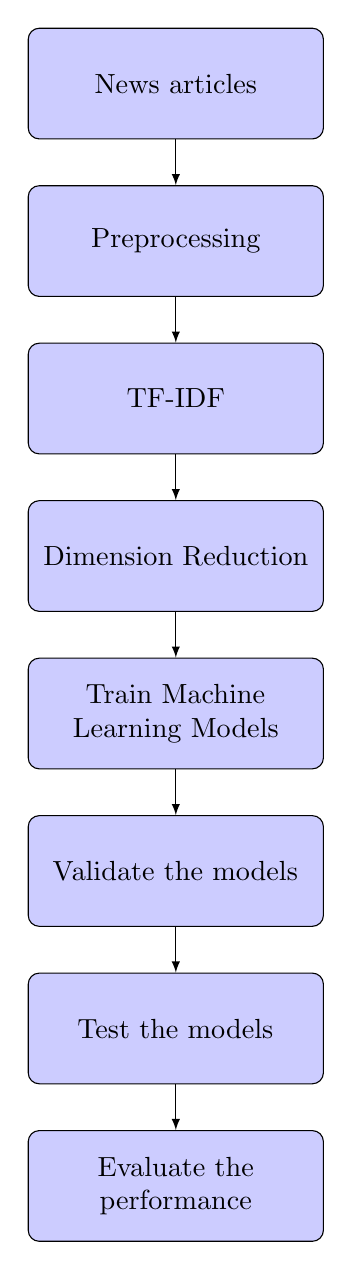
\begin{tikzpicture}[node distance = 2cm, auto]
\node [block] (init) {News articles};
\node [block, below of=init] (preprocessing) {Preprocessing};
\node [block, below of=preprocessing] (tfidf) {TF-IDF};
\node [block, below of=tfidf] (dimred) {Dimension Reduction};
\node [block, below of=dimred] (ml) {Train Machine Learning Models};
\node [block, below of=ml] (validate) {Validate the models};
\node [block, below of=validate] (test) {Test the models};
\node [block, below of=test] (eval) {Evaluate the performance};
% Draw the edges
\path [line] (init) -- (preprocessing);
\path [line] (preprocessing) -- (tfidf);
\path [line] (tfidf) -- (dimred);
\path [line] (dimred) -- (ml);
\path [line] (ml) -- (validate);
\path [line] (validate) -- (test);
\path [line] (test) -- (eval);
\end{tikzpicture}

First, the news articles must undergo preprocessing. The preprocessing includes converting all the words to lowercase, numbers and punctuations removal, stop words removal, stemming and others. 

After preprocessing, TF-IDF algorithm would be applied on the text to extract the features from the text. The resulting vector space from TF-IDF would be undergo a dimension reduction algorithm.

After vector space model dimension is reduced, the vector space model is used to train a machine learning algorithm. The trained machine learning model is validated and tested and its performance is evaluated.

The vector space model of the news articles from TF-IDF can undergo different dimension reduction algorithm or none at all. The classification accuracy stemming from this differences would be compared. 

The machine learning algorithms use to train the models would be the few document classification machine learning algorithms chosen in chapter 2, namely SVM, kNN and Neural Network.

\section{Conclusion}
With the method mentioned above, the experiments would be carry out and the results would be recorded. The results would be compared and the differences would be analysed.
%!TEX ROOT = main.tex

\chapter{Results and Discussions}

\section{Introduction}
The results of the experiments are shown in this section. The differences in the accuracy and performance of each of the methods would be discussed and analysed. Hopefully, the results and discussions would be able to answer the research questions posted in the beginning of this research.

\section{Term frequency}

\begin{table}[ht]
	\centering
	\begin{tabular}{|| c | c | c | c||}
		\hline
		ML & no of features & accuracy & time taken (s) \\ [0.5ex]
		\hline\hline
		kNN & 8000 & 0.31 & 3.74 \\ 
		\hline
		SVM & 8000 & 0.81 & 5.27 \\
		\hline
		NN & 8000 & 0.84 & 91.82 \\
		\hline
	\end{tabular}
\caption{Term frequency}
\label{tbl:termFrequency}
\end{table}

Term frequency is one of most common feature extraction method in text. It convert all the words in the dataset into a matrix where each column is a word and the value in each of the columns are the number of times each word appear in the text. Each row in the matrix is a document. This vector space model representation of the words would result in a sparse matrix since each of the documents only contains a subset of all the words in the whole dataset. 

In this experiment, the number of features of vector space model from term frequency extraction is limited to 8000, this is because of the memory constraint of the machine, if it is unlimited the resulting matrix would be of bigger size and would have the probability of running out of memory while processing the matrix. 

In the results shown above, NN achieved an accuracy of 0.84 which is the best accuracy out of the 3 classification algorithm but it is also the one that takes the longest to process which is 91.82s. kNN took the least time to process, 3.74s but has the lowest accuracy score, 0.31. Overall performance, SVM is the best, it only took 5s to process, which is 80s less than NN and has an accuracy of 0.81 which is comparable with NN. 

reason of KNN accuracy low [reference] [https://arxiv.org/abs/1011.2807]\\
kNN accuracy is low in this scenario is possibly due to the sparsity of the feature matrix or vector space model. The data points are few and far in between. kNN is designed for low dimensional data therefore it doesn't perform well in large and sparse data. The underlying reason would be due to kNN classify a new data point based on the distance of the new data point with the nearby data points. Since the other data points are few and sparse, the classification of the new data points would be biased to the few data points that are near. This bias would reduce the accuracy of the classification.

NN took the longest time to process the features, this is due to the layers of neurons in NN. The vector space model even though sparse has high dimension, NN would need as much if not more neurons as the number of features to process the data. This processing would takes both time and computing power.

SVM depends on the prominent features of the dataset, the support vectors to classify the dataset so it is relatively faster and as accurate.

\clearpage
\section{Term frequency with naive dimension reduction}

\begin{table} [ht]
	\centering
	\begin{tabular}{|| c | c | c | c | c||}
		\hline
		ML & parameter value & no of features & accuracy & time taken (s) \\ [0.5ex]
		\hline\hline
		kNN & 100 & 2530 & 0.34 & 3.94 \\ 
		\hline
		kNN & 500 & 478 & 0.42 & 4.66 \\ 
		\hline
		kNN & 1000 & 173 & 0.41 & 5.17 \\ 
		\hline\hline
		SVM & 10 & 12705 & 0.83 & 6.10 \\
		\hline
		SVM & 100 & 2530 & 0.76 & 5.67 \\
		\hline
		SVM & 500 & 478 & 0.63 & 20.20 \\
		\hline\hline
		NN & 10 & 12705 & 0.87 & 116.78 \\
		\hline
		NN & 100 & 2530 & 0.80 & 48.08 \\
		\hline
		NN & 500 & 478 & 0.65 & 61.87 \\
		\hline
	\end{tabular}
\caption{Term frequency with naive dimension reduction}
\label{tbl:termFrequencyNaive}
\end{table}

The feature extraction method used in this experiment is same as the experiment above but dimension reduction method is applied to the resulting matrix before training. The dimension reduction algorithm used in this experiment is a naive one which means that the columns with the least occurrence of word are removed assuming those words are unimportant and would not have much influence on the accuracy.

The parameter value is just an integer value passed to the dimension reduction function implemented. It has an inversely proportional relationship with the number of features. The larger the parameter value, the more columns would be removed and the number of features would decrease.

In the result table above, each of the classification algorithm has different parameter value, this is determined by trial and error and the results shown are the best.

In this experiment, kNN still has the worst performance among the 3 which is at 0.34 with 2530 number of features. As the number of features decreases to 173, the accuracy increases slightly to 0.41. As the number of features decreases, the time taken for kNN to produce the result increases from 3.946s to 5.17s.

SVM and NN have the same trend in this experiment, the accuracy and time taken decrease as the number of features decreases. Accuracy of SVM decreases from 0.83 to 0.63 as the number of features decreases from 12705 to 478. The time taken by SVM as increases from 6.1s to 20.20s as the number of features decrease drastically. The decrement in accuracy in SVM is slight in relative to the decrement in the number of features. Accuracy decreased by 0.20 while the number features has decreased by 12227.

The time taken by SVM increases quite drastically when the number of features decreased. The sparsity of the vector space model decreases, resulting in a denser vector space model. SVM need to take into account more data points to calculate an effective hyperplane to separate the data points into different classes.

On the other hand, the accuracy of NN decreases from 0.87 to 0.65 as the number of features decreased from 12705 to 478. However, the time taken by NN decreases from 116.78s to 61.87s. The decrement in time taken is possibly due to the reduction of features, less neurons are needed to process the data and thus the speedup.

In the scenarios where SVM and NN have more features than the first experiment with just term frequency, both of the classification algorithms have better accuracy. These 2 classification algorithms are efficient and able to process features in a large and sparse vector space.


\clearpage
\section{Term frequency with SVD}

\begin{table} [ht]
	\centering
	\begin{tabular}{|| c | c | c | c||}
		\hline
		ML & no of features & accuracy & time taken (s) \\ [0.5ex]
		\hline\hline
		kNN & 4000 & 0.31 & 482.66 \\
		\hline
		kNN & 2000 & 0.38 & 216.59 \\ 
		\hline
		kNN & 500 & 0.49 & 60.89 \\ 
		\hline
		kNN & 100 & 0.55 & 15.38 \\ 
		\hline
		kNN & 10 & 0.30 & 2.78 \\ 
		\hline\hline
		SVM & 4000 & 0.80 & 370.43 \\
		\hline
		SVM & 2000 & 0.78 & 172.58 \\
		\hline
		SVM & 500 & 0.77 & 85.03 \\
		\hline\hline
		NN & 4000 & 0.80 & 220.76 \\
		\hline
		NN & 2000 & 0.79 & 91.13 \\
		\hline
		NN & 500 & 0.77 & 40.86 \\
		\hline
	\end{tabular}
\caption{Term frequency with SVD}
\label{tbl:termFrequencySvd}
\end{table}

In this experiment, the feature extraction or document representation method used is still term frequency but the dimension reduction algorithm has been changed. Instead of reducing the dimension of the feature matrix naively by removing the terms that has the lowest frequency, SVD is used. SVD would reduce the dimension of the vector space model by retrieving the features with maximum variance in the data.

The number of features shown in the table above is the number of columns in the resulting matrix after applying SVD.

Similar with the trend in the previous experiment (term frequency with naive dimension reduction), the accuracy of kNN increases slightly, from 0.34 to 0.38 when the features decreases from 4000 to 2000, but the resulting accuracy is still far from satisfactory. The time taken by kNN decreases from 482s to 216s as the number of features decreases. Since kNN is dependent on the calculation of Euclidean distance between the data points, processing a less sparse matrix would be more efficient.

The accuracy of SVM and NN also have the same trend with the previous experiment, the accuracy decreases slightly when the number of features decreases. Accuracy of SVM decreases from 0.80 to 0.78 and the accuracy of NN decreases from 0.80 to 0.79 as the number of features decreases from 4000 to 2000.

As expected, the time taken by the classification model to reduce the dimension and predict the result decreases as the number of features decreases. However, in comparison with the time taken in the previous experiments, the time taken in this experiment is astoundingly higher, the time taken by SVM and NN increase by 365s and 130s respectively when SVD is applied. SVD would be the culprit, dimension reduction comes at a cost which is processing power. To reduce or compress the features into a small dimension, a lot of calculation would be involved, this would take both time and processing power.

The resulting accuracy is not as good as just with term frequency. This is expected because the number of features decreased. The reduction in features may save some memory space but in order to achieve that more processing power and time would be needed.

Comparing the performance of the classification models in this experiment with the second experiment, term frequency with naive dimension reduction, the performance of the classification models are almost similar. This comparison is made on the scenarios where the same classification model has the almost the same number of features, namely 2530 on the second experiment and 2000 in this experiment. This is unexpected, the assumption before was SVD is a better dimension reduction algorithm than naive dimension reduction. The resulting vector space model from SVD should contains the maximum variance of the data, the classification models trained with this model should have a better performance than the models trained with naive dimension reduction.

This experiment show that this is not the case. The different dimension reduction algorithm produces almost similar accuracy with term frequency document representation method. The underlying problem of this issue maybe is the document representation method rather than the dimension reduction. Therefore, the following experiments would apply a different document representation algorithm.\\

\clearpage
\section{TF-IDF}

\begin{table} [ht]
	\centering
	\begin{tabular}{|| c | c | c | c||}
		\hline
		ML & no of features & accuracy & time taken (s) \\ [0.5ex]
		\hline\hline
		kNN & 8000 & 0.76 & 3.71 \\ 
		\hline
		SVM & 8000 & 0.87 & 2.39 \\
		\hline
		NN & 8000 & 0.88 & 55.82 \\
		\hline
	\end{tabular}
\caption{TF-IDF}
\label{tbl:tfidf}
\end{table}

The findings from the previous experiments show that the different reduction algorithms produce similar accuracy which is contradictory to the hypothesis or assumption that the SVD would obtain a better performance out of the classification models. To investigate this hypothesis further, a different document representation algorithm is applied.
 
The document representation algorithm applied in this experiment and the following experiment is TF-IDF. In contrast with term frequency which only take the frequency of each word into account, TF-IDF takes both the frequency of each word and the rarity of it into account. If a term or word appear in high frequency but in many documents, this word may not be of importance and consequently is not a meaningful feature. If a word appear rarely and only in a few documents, this word would have high importance and would be meaningful feature of the few documents.

With TF-IDF, kNN can achieved a satisfactory accuracy score of 0.76 even though the number of features in the resulting matrix of TF-IDF is the same with term frequency which is 8000. The vector space model of TF-IDF would not be as sparse as that of term frequency which is kNN is more suitable for kNN.

NN is still provide the highest accuracy score of 0.88 but the time taken also the longest at 55.82s.

SVM achieved an accuracy of 0.87 which is just 0.01 shy of what achieved by NN and the time taken is the lowest among the 3 which is 2.39s.

In comparison with the first experiment that apply term frequency document representation without dimension reduction, the performance of the classification models significantly improve. kNN accuracy has more than doubled from 0.31 to 0.76. SVM accuracy increases from 0.81 to 0.87 while accuracy of NN increases from  0.84 to 0.88. Besides accuracy, the time taken also improved, time taken by SVM reduces from 5.27s to 2.39s while time taken by NN reduces from 91.82s to 55.82s. All these improvements are achieved with the same number of features in the vector space, which is 8000. 

The performance of the classification models in this experiment is also better than the those in the 2 experiments above with dimension reduction. However this may not be a fair comparison because the different number of features are used and dimension reductions are not applied in this experiment. Dimension reduction algorithms would be applied to the vector space model resulting from TF-IDF in the following experiments in order to have a fair comparison.

The performance increment from term frequency to TF-IDF seems to prove that TF-IDF is a better document representation method.\\

\clearpage
\section{TF-IDF with naive dimension reduction}

\begin{table} [ht]
	\centering
	\begin{tabular}{|| c | c | c | c | c||}
		\hline
		ML & parameter value & no of features & accuracy & time taken (s) \\ [0.5ex]
		\hline\hline
		kNN & 50 & 4221 & 0.74 & 4.00 \\ 
		\hline
		kNN & 100 & 2530 & 0.71 & 4.11 \\ 
		\hline
		kNN & 500 & 478 & 0.49 & 5.15 \\ 
		\hline\hline
		SVM & 50 & 4221 & 0.86 & 2.58 \\
		\hline
		SVM & 100 & 2503 & 0.83 & 2.63 \\
		\hline
		SVM & 500 & 478 & 0.66 & 2.94 \\
		\hline\hline
		NN & 50 & 4221 & 0.85 & 38.80 \\
		\hline
		NN & 100 & 2530 & 0.83 & 34.28 \\
		\hline
		NN & 500 & 478 & 0.64 & 77.12 \\
		\hline
	\end{tabular}
\caption{TF-IDF with naive dimension reduction}
\label{tbl:tfidfNaive}
\end{table}

Similar with the experiment with term frequency, naive dimension reduction is applied to the vector space model generated from TF-IDF. The trend over all the 3 machine learning models when the number of features decreases are similar. The accuracy of the classification models decreases and the time taken increases. 

The accuracy achieved by kNN with TF-IDF plus naive dimension reduction is still passable at 0.74 when the features reduced from 8000 to 4221. kNN's accuracy dropped slightly to 0.71 when the number of features decreases to 2530. When the number of features decreases from 2530 to 478, as expectedly the accuracy of kNN dropped for quite a large margin, from 0.71 to 0.49. The time taken by kNN increases slightly from 4s to 5s as the features decreases.

SVM has the same behaviour with kNN in this experiment, its accuracy decreases from 0.86 to 0.83 and then to 0.66 when the number of features decreases from 4221 to 2503 to 478. The time taken increases slightly as well as the number of features decreases.

NN also has the similar trend in accuracy as the number of features decreases. NN's accuracy decreases from 0.85 to 0.64 when the number of features decreases from 4221 to 478. The differences in NN is that the time taken almost doubled when the number of features is low compare to when the number of features is high. The time taken is 38s when there is 4221 features and when there is only 478 features, the time taken doubled to 77s.

In the scenarios where the number of features are almost halved, from 8000 to 4221, the performance of the classification models are still comparable with the performance achieved with just TF-IDF without any dimension reduction. The accuracy are almost the same, the time taken is similar except NN which has quite a speedup when the number of features is reduced to 4221.

It can be deduced that with naive dimension reduction, the number of features and memory needed to store the vector space model is reduced. With this reduced number of features, the classification models can still achieve comparable performance at a slightly decreased capacity.

This is mainly because of the reduction in features. As the amount of information became lesser, less information is available to train a comprehensive model. Therefore, the accuracy of the models decrease. Even though the dimension reduction applied is a naive one and less computing intensive, it still increases the time taken compared with just with TF-IDF. The more reduction is performed, the time taken would increase as well.

\clearpage
\section{TF-IDF with SVD}

\begin{table} [ht]
	\centering
	\begin{tabular}{|| c | c | c | c||}
		\hline
		ML & no of features & accuracy & time taken (s) \\ [0.5ex]
		\hline\hline
		kNN & 4000 & 0.77 & 457.16 \\
		\hline
		kNN & 2000 & 0.58 & 208.64 \\ 
		\hline
		kNN & 500 & 0.55 & 58.58 \\ 
		\hline
		kNN & 100 & 0.69 & 15.09 \\
		\hline
		kNN & 50 & 0.69 & 7.58 \\ 
		\hline
		kNN & 10 & 0.55 & 2.54 \\ 
		\hline\hline
		SVM & 4000 & 0.87 & 189.32 \\
		\hline
		SVM & 2000 & 0.86 & 69.63 \\
		\hline
		SVM & 500 & 0.83 & 19.59 \\
		\hline\hline
		NN & 4000 & 0.85 & 215.73 \\
		\hline
		NN & 2000 & 0.84 & 87.12 \\
		\hline
		NN & 500 & 0.81 & 56.60 \\
		\hline
	\end{tabular}
\caption{TF-IDF with SVD}
\label{tbl:tfidfSvd}
\end{table}

Finally, this experiment is applying SVD dimension reduction to the resulting vector space model from TF-IDF. Similar with experiment before that apply SVD, each of the classification models would be tested with 2 set of vector space model, each with different number of features, namely 2000 and 4000. To put it in perspective, the number of features without reduction is 8000. 

When the number of features are at 4000 which is halved, kNN still can produced an accuracy of 0.77 which is similar with what is achieved with TF-IDF without dimension reduction. Same goes to SVM and NN, at 4000 features, the accuracy are quite similar with TF-IDF without dimension reduction. However, when the dimension of the vector space model is reduced to 2000, the accuracy across 3 of the classification models dropped. kNN being the most drastic, its accuracy dropped to 0.58 while SVM and NN dropped to 0.86 and 0.84 respectively, which is slightly worse than before but it is still satisfactory.

Comparing with the results of the experiment with TF-IDF and naive dimension reduction, this performance of the classification models with SVD has a slight advantage. The accuracy is slightly better with SVD rather than with naive dimension reduction. This would be due to the advantage of SVD obtaining the maximum variance of the features over naive dimension reduction, even though the increment over accuracy is slight.

There is an odd trend on the time taken for all 3 classification models though. The time taken in this experiment is much higher than the experiment of TF-IDF without dimension reduction and TF-IDF with naive dimension reduction which is expected. This would be due to SVD reduction takes more time as more calculation is needed. However, the time taken decreased when the further reduction is done, kNN take 457s to reduce the vector space model from 8000 to 4000 but just 208s to reduce the vector space model from 8000 to 2000. Keep in mind that the time recorded here includes the time taken for the classification model to predict the test dataset as well. This trend appear in SVM and NN as well. SVM took 189s to reduce 8000 to 4000 but just 69s to reduce 8000 to 2000 while NN took 215s to reduce 8000 to 4000 and 87s to reduce 8000 to 2000. 

The decrement in time could be explained with the reduction of features, the time taken to process them also reduced. Therefore it provided a speedup. This speedup that comes with the reduction of features, comes at a cost which is accuracy. For SVM and NN, the reduction in accuracy is meagre thus it would be logical to trade the slight accuracy with the speedup but in kNN the trade off would be lopsided in the favour of time taken.

\clearpage
\section{Conclusion}
From the results of the 6 experiments above, it is found that TF-IDF is a better document representation algorithm than term frequency. The resulting vector space model from TF-IDF can achieve a higher accuracy than that of term frequency. 

The effect of dimension reduction on the accuracy of the classification models is analysed. Dimension reduction, naive and otherwise, do reduce the dimension of the vector space model, reducing the memory needed to store the matrix. However, this reduction in features and information would result in a loss of accuracy. SVD would be a better dimension reduction algorithm compared to the naive method because the accuracy achieved with SVD is slightly higher than that of naive method.

Out of the 3 classification models tested in the experiments, SVM is the most efficient and versatile. SVM can achieve high accuracy (> 0.80) in most scenarios. NN can also achieve high accuracy in most of the cases tested but NN took the longest time. SVM has an advantage over NN with the processing time. Therefore, SVM would be the most efficient text classification model among the 3 classification models.


%!TEX ROOT = main.tex
\chapter{Conclusion}
It is known that \ac{tfidf} should be better than term frequency but Moldagulova, Aiman and Sulaiman, Rosnafisah proposed that with term frequency and naive dimension reduction, \ac{knn} classification model would be able to achieve a satisfactory result. \cite{knnVectorSpaceReduction}. Therefore, this research compare term frequency and \ac{tfidf} and apply different dimension reduction methods to both. The implementation of the \ac{knn} algorithm in this research might differ from that proposed by the authors. They divided the larger feature matrix into parts and train by part.

From the results of the experiments it is shown that \ac{tfidf} is a better document representation method than term frequency. Classification models can achieved a better result with \ac{tfidf} than term frequency. With term frequency as the document representation method, \ac{svm} and \ac{nn} are able to achieve satisfactory accuracy but the accuracy achieved with \ac{tfidf} is slightly higher. The advantage of \ac{tfidf} is more obvious, with \ac{knn}, with term frequency the accuracy is a meagre 0.31 but with \ac{tfidf}, the accuracy is 0.76 which is close to 0.80.

By applying the 2 types of dimension reduction to both the document representation method, the effect of dimension reduction on the performance of the classification models is analysed. The classification models accuracy from both naive dimension reduction and truncated \ac{svd} are quite similar in most cases. However, truncated \ac{svd} has a slight edge over naive dimension reduction. Truncated \ac{svd} can provide classification models with more prominent features and subsequently higher accuracy.

As the dimension of the vector space model is reduced, the accuracy of the classification models would decreased due to the lack of features or information. This reduction of features would reduce the memory used to store the vector space model. However, the reduction process would need intensive computing power and time, especially in the case of truncated \ac{svd}. This the trade off between dimension reduction and classification accuracy. The gain in less memory to store the matrix would cause an increase in computing power consumed and time taken.

Out of the 3 classification models tested in this research, \ac{svm} has the best overall performance. \Ac{svm} can achieve a satisfactory accuracy in most scenarios and the time taken for \ac{svm} to predict the test data is among the shortest. Thus \ac{svm} would be the best classification models in text classification.

For future works, ways to improve the accuracy of the classification models with \ac{tfidf} should be explored. More document representation method, such as n-gram could be apply alongside \ac{tfidf} and different dimension reduction could be applied. \Ac{tfidf} does not take the semantic of the term into account just the frequency and rarity, n-gram would be able to rectify part of the problem.\\


\bibliography{myrefs}

\begin{appendices}
%!TEX ROOT = main.tex
\chapter{Data preprocessing implementation}
The code in this section show how the 20 news group dataset is processed before it is used to train classification models.\\

\lstinputlisting[language=python]{PreparingDataset.py}

\chapter{Data Exploratory Implementation}
The code below is used to check the distribution of the categories in the dataset.\\

\lstinputlisting[language=python]{DataExploratory.py}

\chapter{Feature extraction and dimension reduction implementation}
The code shown in this section is the code that used to generate the feature matrix and apply the dimension reduction to the feature matrix.\\

\lstinputlisting[language=python]{GenTfIdf.py}

\chapter{kNN classification model implementation}
The code for kNN classification model is shown below.\\

\lstinputlisting[language=python]{20newsKNN.py}

\chapter{SVM classification model implementation}
SVM classification model implementation is shown as follows.\\

\lstinputlisting[language=python]{20newsSVM.py}

\chapter{NN classification model implementation}
NN classification model implementation is shown as follows.\\

\lstinputlisting[language=python]{20newsNN.py}

\end{appendices}

\end{document}
